%%%%%%%% ICML 2026 Workshop Submission - 4-page short paper format %%%%%%%
% Structure modeled on NeurIPS MATH-AI 2024 short papers and
% ICML AI4Math 2024 short-track papers (Abstract / Intro / Method /
% Results / Discussion in 4 pages, with unlimited refs and appendix).

\documentclass{article}

\usepackage{microtype}
\usepackage{graphicx}
\usepackage{booktabs}
\usepackage[hidelinks]{hyperref}
\hypersetup{colorlinks=true, allcolors=black, pdfborder={0 0 0}}
\usepackage{amsmath}
\usepackage{amssymb}
\usepackage{mathtools}
\usepackage{xcolor}
\usepackage{tikz}
\usetikzlibrary{arrows.meta,positioning,calc,shapes,fit,backgrounds}
\usepackage[capitalize,noabbrev]{cleveref}
\usepackage{multirow}
\usepackage{enumitem}
\usepackage{listings}
\lstdefinestyle{xsgrv}{
  basicstyle=\ttfamily\scriptsize\color{black},
  keywordstyle=\color{black},
  commentstyle=\color{black},
  stringstyle=\color{black},
  identifierstyle=\color{black},
  numbers=none,
  frame=single,
  framesep=3pt,
  framexleftmargin=2pt,
  framexrightmargin=2pt,
  rulecolor=\color{black},
  breaklines=true,
  breakatwhitespace=true,
  postbreak=\mbox{\textcolor{black}{$\hookrightarrow$}\space},
  showstringspaces=false,
  columns=fullflexible,
  keepspaces=true,
  xleftmargin=0pt,
  xrightmargin=0pt,
  linewidth=\linewidth,
  resetmargins=true,
  language=Python,
}

\usepackage{icml2026}
\icmltitlerunning{Cross-Family Symbolic Verification}

\begin{document}

\twocolumn[
\icmltitle{Cross-Family Symbolic Verification for \\
Contamination-Robust Selective Prediction on LLM Math Reasoning}

\begin{icmlauthorlist}
\icmlauthor{Anonymous Authors}{anon}
\end{icmlauthorlist}
\icmlaffiliation{anon}{Anonymous submission to an ICML 2026 workshop.}
\icmlcorrespondingauthor{Anonymous Authors}{anonymous@example.org}
\icmlkeywords{Selective Prediction, Math Reasoning, Verification, Contamination, LLM}

\vskip 0.3in
]

\printAffiliationsAndNotice{}

\begin{abstract}
Selective prediction for LLM math reasoning fails along two coupled axes: same-model self-verification suffers correlated-error collapse (13.8\% false acceptance on MATH-500, scaling monotonically from 1.4\% at Level~1 to 30.8\% at Level~5), and agreement-based signals look strong on MATH-500 but collapse on benchmarks released after the solver's training cutoff. We introduce \textbf{X-SGRV}, in which a large LLM from a different family than the solver reads only the problem statement and emits a SymPy \texttt{verify(answer)} function executed in a sandboxed subprocess; a gold-free adversarial filter and cross-extractor consensus eliminate residual false positives. On the pre-registered full MATH-500 ($n{=}498$), strict two-way consensus accepts $171$ candidates and is correct on all $171$ (95\% Clopper-Pearson CI $[0.979,1.000]$) at 34.3\% coverage. On contamination-clean AIME 2025 and a 125-problem post-cutoff combo, coverage correctly collapses to 3--12\% while accepted answers remain right. At matched coverage X-SGRV ties Skywork-o1-Open-PRM and doubles Qwen-Math-PRM on the contamination-clean combo.
\end{abstract}

%==============================================================================
\section{Introduction}
%==============================================================================

Selective prediction on LLM math reasoning needs a deployment-time signal indicating which answers should be trusted. Two coupled failure modes obstruct this. First, same-model self-verification is correlated by construction: when the solver also writes the assertions checking its work, errors in the solution propagate into the assertions, and the verifier inherits the solver's blind spots~\citep{huang2024selfcorrect,kim2025correlated,stechly2024selfverify}. Second, MATH-500 is partially memorized by the standard solvers used to study it: Qwen2.5-Math-7B reproduces 54.6\% of the benchmark verbatim from a 60\% prefix, with accuracy dropping sharply on post-cutoff problems~\citep{wu2025contam}. High top-tier precision on MATH-500 therefore confounds verification reliability with memorization.

Three prior lines address one failure but not both. Code-based same-model self-verification~\citep{mathcoder2024,mathshepherd2024} is executable but does not break the solver/verifier coupling. Process reward models~\citep{lightman2024prm,qwenprm2025,skyworkprm2024} inherit the contamination footprint of their training distribution. Autoformalization checks~\citep{dtv2024} achieve structural independence but require heavyweight formal-methods infrastructure with reported coverage below 20\% on competition problems.

\textbf{Contribution.} We introduce X-SGRV (\Cref{fig:pipeline}), in which a large LLM from a different model family than the solver reads only the problem statement and emits a Python \texttt{verify(answer)} function executed in a SymPy sandbox. A gold-free deployment-time adversarial filter probes the verifier against perturbations of the candidate; cross-extractor consensus requires multiple independent extractors to all produce working verifiers and all accept. On the pre-registered full MATH-500, strict two-way consensus is correct on $171/171$ accepts ($[0.979,1.000]$) at 34.3\% coverage; on contamination-clean benchmarks the system correctly collapses to single-digit coverage while preserving precision; at matched coverage it ties Skywork-PRM and doubles Qwen-PRM on the contamination-clean combo, while requiring no GPU infrastructure.

%==============================================================================
\section{Method}
\label{sec:method}
%==============================================================================

\begin{figure}[t]
\centering
\resizebox{\columnwidth}{!}{%
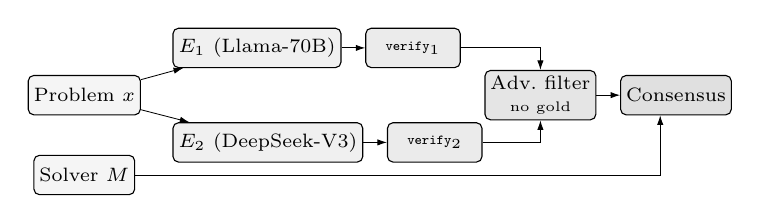
\begin{tikzpicture}[
  node distance=2mm and 3mm,
  every node/.style={font=\scriptsize},
  box/.style={draw, rounded corners=2pt, inner sep=2pt, minimum height=5mm,
              align=center, line width=0.4pt},
  prob/.style={box, fill=gray!8, minimum width=11mm},
  ext/.style={box, fill=gray!12, minimum width=17mm},
  ver/.style={box, fill=gray!16, minimum width=12mm, font=\ttfamily\tiny},
  filt/.style={box, fill=gray!20, minimum width=13mm},
  cons/.style={box, fill=gray!24, minimum width=11mm},
  sol/.style={box, fill=gray!8, minimum width=11mm},
  arr/.style={-{Latex[length=1.2mm,width=0.8mm]}, line width=0.3pt},
]
  \node[prob] (p) {Problem $x$};
  \node[ext, right=4mm of p, yshift=6mm]  (e1) {$E_1$ (Llama-70B)};
  \node[ext, right=4mm of p, yshift=-6mm] (e2) {$E_2$ (DeepSeek-V3)};
  \node[ver, right=3mm of e1] (v1) {verify$_1$};
  \node[ver, right=3mm of e2] (v2) {verify$_2$};
  \node[filt, right=3mm of v1, yshift=-6mm] (f) {Adv.\ filter\\{\tiny no gold}};
  \node[cons, right=3mm of f] (c) {Consensus};
  \node[sol, below=5mm of p] (s) {Solver $M$};
  \draw[arr] (p) -- (e1); \draw[arr] (p) -- (e2);
  \draw[arr] (e1) -- (v1); \draw[arr] (e2) -- (v2);
  \draw[arr] (v1) -| (f); \draw[arr] (v2) -| (f);
  \draw[arr] (f) -- (c);
  \draw[arr] (s.east) -| ([xshift=-2mm]c.south);
\end{tikzpicture}%
}
\caption{\textbf{X-SGRV pipeline.} Independent cross-family extractors $E_1,E_2$ read the problem statement only and emit SymPy \texttt{verify} functions. The deployment-time filter probes each verifier against perturbations $\{\hat a\pm 1,\hat a+7,\hat a\times 2\}$ of the solver's candidate $\hat a$; verifiers accepting any probe are marked broken. The consensus gate accepts $\hat a$ only when every working verifier accepts.}
\label{fig:pipeline}
\end{figure}

A solver $M$ produces a plurality candidate $\hat a$ for problem $x$. A cross-family extractor $E$, drawn from a model family architecturally distinct from $M$, receives only $x$ and emits a Python function \texttt{verify(answer) -> bool} that re-derives the problem's constraints from the statement in SymPy plus standard library primitives. The prompt forbids hard-coding the answer and requires the literal token \texttt{UNVERIFIABLE} when no bounded check is possible.

The emitted script is executed in a Python subprocess sandbox with a 10-second \texttt{SIGALRM} timeout. The deployment-time adversarial filter probes each verifier against $\mathcal{P}(\hat a) = \{\hat a-1,\hat a+1,\hat a+7,\hat a\times 2\}$ (for integer $\hat a$; deterministic fallback for non-integers). A verifier that accepts any probe is marked broken. Strict $k$-way cross-extractor consensus accepts $\hat a$ only when every participating extractor produces a working verifier and every working verifier accepts. The probe set and consensus rule were locked in a pre-registration document committed before the $n{=}498$ scale-up. Implementation details, full extractor prompt, baseline configurations, and statistical methodology are in \Cref{app:methods,app:stats}.

%==============================================================================
\section{Experiments}
\label{sec:exp}
%==============================================================================

\textbf{Setup.} Solver: \texttt{Qwen2.5-7B-Instruct-Turbo} (Together AI). Extractors: \texttt{Llama-3.3-70B}, \texttt{DeepSeek-V3}, \texttt{gpt-oss-120b}, \texttt{Claude Sonnet 4.6}, \texttt{Qwen3-Coder-480B}. Benchmarks: full MATH-500 ($n{=}498$ after solver timeouts), stratified MATH-500 ($n{=}175$, balanced across Levels 1--5), AIME 2025 ($n{=}30$), and a CleanMath combo of HMMT-Feb/BRUMO/SMT/APEX 2025 ($n{=}125$). Baselines: 4/10-sample self-consistency~\citep{wang2023selfconsistency}, semantic entropy~\citep{kuhn2023semantic,farquhar2024nature}, $p(\textsc{True})$~\citep{kadavath2022}, \texttt{Qwen2.5-Math-PRM-7B}~\citep{qwenprm2025} and \texttt{Skywork-o1-Open-PRM-7B}~\citep{skyworkprm2024} run on Modal A100; PRMs validated against ProcessBench~\citep{processbench2024}.

\textbf{Same-model FAR scales with difficulty.} Same-model SymPy self-verification accepts $320$ MATH-500 candidates with a $13.8\%$ false acceptance rate, scaling monotonically from $1.4\%$ at Level~1 to $30.8\%$ at Level~5; a 2$\times$2 ablation isolates solver-verifier \emph{independence}, not test-input randomization, as the operative axis (Fisher's exact $p<10^{-8}$; \Cref{app:results}).

\textbf{Single-extractor X-SGRV.} On the full MATH-500 ($n{=}498$), a Llama-3.3-70B extractor accepts $243$ candidates and is correct on $230$, precision $0.947$ ($[0.91, 0.97]$) at 48.8\% coverage with zero gold-relative adversarial false positives over $964$ probes. A DeepSeek-V3 extractor reaches $199/207 = 0.961$ ($[0.93, 0.98]$) at 41.6\% coverage.

\textbf{Cross-extractor consensus drives residual FPs to zero (\Cref{tab:main}).} Strict two-way consensus (Llama $\cap$ DeepSeek-V3) on the pre-registered full MATH-500 accepts $171$ candidates and is correct on all $171$ (95\% CI $[0.979, 1.000]$) at 34.3\% coverage. Adding three further extractors --- gpt-oss-120b, Claude Sonnet 4.6, Qwen3-Coder-480B --- to form a five-way consensus on stratified MATH-175 yields $69/69 = 1.000$ ($[0.948, 1.000]$). Adding a sixth extractor (GPT-5-mini) reduces the accepted tier to $67/67 = 1.000$ ($[0.946, 1.000]$). Adding extractors monotonically shrinks the accepted tier while preserving perfect precision.

\textbf{Coverage correctly collapses on contamination-clean benchmarks.} On AIME 2025 the deployment-time filter removes the single broken verifier and yields $1/1 = 1.000$ at 3.3\% coverage; on CleanMath the system abstains on $121/125$ problems and accepts $4$ correct candidates (precision $1.000$). A rotated solver (DeepSeek-V3.1) raises the CleanMath accept count to $15/15$, isolating the verifier's selectivity from solver accuracy.

\textbf{Matched-coverage comparison against PRMs (\Cref{tab:prm}).} At 54.9\% coverage on MATH-175, X-SGRV, Qwen-PRM (min-step), and Skywork-PRM (product-step) all achieve precision $0.927$--$0.938$; on the contamination-clean CleanMath at 3.2\% coverage, X-SGRV and Skywork-PRM (mean-step) reach $4/4 = 1.000$ while Qwen-PRM (min-step) reaches $2/4 = 0.500$, a split consistent with Qwen-PRM's training distribution being more concentrated on MATH-family problems.

\begin{table}[t]
\centering
\caption{\textbf{X-SGRV top-tier precision across extractors, benchmarks, and consensus configurations.} ``Cov.'' is the size of the top tier; ``Prec.'' is 95\% Clopper-Pearson. CleanMath = HMMT-Feb + BRUMO + SMT + APEX 2025 ($n{=}125$).}
\label{tab:main}
\resizebox{\columnwidth}{!}{%
\begin{tabular}{llrl}
\toprule
Extractor & Benchmark & Cov. & Prec.\ (95\% CI) \\
\midrule
Llama-3.3-70B    & MATH-500    & 48.8\% & 230/243 = 0.947 \\
DeepSeek-V3      & MATH-500    & 41.6\% & 199/207 = 0.961 \\
Claude Sonnet 4.6& AIME 2025   & 10.0\% & 3/3 = 1.000 \\
Llama-3.3-70B    & CleanMath   & 3.2\%  & 4/4 = 1.000 \\
\midrule
2-way consensus  & MATH-500    & 34.3\% & 171/171 = 1.000 \\
5-way consensus  & MATH-175    & 39.4\% & 69/69 = 1.000 \\
\midrule
Llama (Solver: DeepSeek-V3.1) & CleanMath & 12.0\% & 15/15 = 1.000 \\
Llama-3.3-70B    & Omni-MATH hard-100 & 1.0\% & 0/1 = 0.000 \\
\bottomrule
\end{tabular}%
}
\end{table}

\begin{table}[t]
\centering
\caption{\textbf{X-SGRV versus open PRMs at matched coverage.}}
\label{tab:prm}
\resizebox{\columnwidth}{!}{%
\begin{tabular}{llrl}
\toprule
Method & Benchmark & Cov. & Prec.\ (95\% CI) \\
\midrule
X-SGRV               & MATH-175 & 54.9\% & 0.938 [0.87, 0.98] \\
Qwen-PRM (min)       & MATH-175 & 54.9\% & 0.927 [0.86, 0.97] \\
Skywork-PRM (prod.)  & MATH-175 & 54.9\% & 0.938 [0.87, 0.98] \\
\midrule
X-SGRV               & CleanMath & 3.2\% & 1.000 [0.40, 1.00] \\
Qwen-PRM (min)       & CleanMath & 3.2\% & 0.500 [0.07, 0.93] \\
Skywork-PRM (mean)   & CleanMath & 3.2\% & 1.000 [0.40, 1.00] \\
\bottomrule
\end{tabular}%
}
\end{table}

%==============================================================================
\section{Discussion}
%==============================================================================

The 22-fold scaling of same-model false acceptance from L1 to L5 is consistent with correlated-error collapse: when one model produces both the solution and the assertions checking it, the assertions describe the model's misreading of the problem~\citep{kim2025correlated}. Specification grounding, by deriving the check from the problem statement, breaks this overlap. The 2$\times$2 ablation shows the operative axis is solver-verifier independence, not test-input randomization (\Cref{app:results}).

Under approximate independence between cross-family extractors, the joint false-positive rate is bounded above by the product of per-extractor rates: empirically $0.053 \times 0.039 \approx 0.002$, consistent with the observed $0/171$. The mechanism is lab-agnostic: five extractors drawn from Meta, DeepSeek, OpenAI, Anthropic, and Alibaba agree on $69/69$ accepts.

X-SGRV is not a continuous-score selective-prediction signal. Top-tier coverage on contamination-clean benchmarks is single-digit by design; on the hardest 100 Omni-MATH problems zero working verifiers are produced, and on PutnamBench-style proof problems the extractor self-detects scope by emitting \texttt{UNVERIFIABLE} on roughly half of a 100-problem sample. The intended deployment posture is escalation, not commitment, when the verifier abstains. Three concrete falsifiable follow-ups: a contamination-stratified replication with per-problem prefix-completion overlap; an extractor-scaling sweep at 13B/32B/70B; and a hybrid SymPy-plus-Lean pipeline (78.9\% Lean compile rate observed for Claude Sonnet 4.6 against Mathlib).

\section*{Reproducibility statement}
All models are public via Together AI, OpenAI, Anthropic, or HuggingFace. The X-SGRV implementation, sandbox harness, adversarial filter, full extractor prompt, result JSONs, and pre-registration document are provided in the anonymized supplementary code release.

\bibliographystyle{icml2025}
\bibliography{references}

\end{document}
